\documentclass[a4paper,11pt,notitlepage]{report}

\usepackage{graphicx}
\usepackage[utf8]{inputenc}
\usepackage[T1]{fontenc}
\usepackage[ngerman]{babel}
\usepackage{bibgerm}
\usepackage{amsmath,amssymb,amsthm}
\usepackage{color}
\usepackage{enumerate}
\usepackage{tabularx}
\usepackage{subfig}
\usepackage{fancyhdr}
\usepackage{upgreek}
\usepackage[pdftex,pdfpagelabels,colorlinks,backref,pagebackref]{hyperref}
\usepackage{tikz} % SELBST HINZUGEFÜGT
\usepackage{lmodern}
\usepackage{subfig}
\usepackage{stmaryrd}
% == Set the heading style ===================================================
\setlength{\headheight}{14pt}
\pagestyle{fancyplain}
\renewcommand{\chaptermark}[1]{\markboth{#1}{}}
\renewcommand{\sectionmark}[1]{\markright{\thesection\ #1}}
\lhead[\fancyplain{}{\thepage}]{\fancyplain{}{\rightmark}}
\rhead[\fancyplain{}{\leftmark}]{\fancyplain{}{\thepage}}
\cfoot{}
\renewcommand{\headrulewidth}{0.4pt}
% ============================================================================

% == Set correct values for fitting floats ===================================
\tolerance=2000
\emergencystretch=10pt

\setcounter{topnumber}{3}
\setcounter{totalnumber}{5}
\setcounter{bottomnumber}{2}

% To make those darn floats fit where they should
\setcounter{totalnumber}{9}
\setcounter{topnumber}{9}
\setcounter{bottomnumber}{9}
\renewcommand{\textfraction}{0.00}
\renewcommand{\topfraction}{1.0}
\renewcommand{\bottomfraction}{1.0}
% ============================================================================

% == German definitions for theorems etc. ==================================== 
\newtheorem{definition}{Definition}[chapter]
\newtheorem{theorem}{Satz}[chapter]
\newtheorem{lemma}{Lemma}[chapter]
\newtheorem{proposition}{Proposition}[chapter]
\newtheorem{corollary}{Korollar}[chapter]
\newtheorem{observation}{Beobachtung}[chapter]
\newtheorem{fact}{Fakt}[chapter]
\newtheorem{remark}{Bemerkung}[chapter]
\newtheorem{example}{Beispiel}[chapter]
% ============================================================================

% == Abkürzungen für die reellen, natürlichen, ganzen,... Zahlen =============
\newcommand{\R}{{\ensuremath{\mathbb{R}}}}
\newcommand{\N}{{\ensuremath{\mathbb{N}}}}
\newcommand{\Z}{{\ensuremath{\mathbb{Z}}}}
\newcommand{\C}{{\ensuremath{\mathbb{C}}}}
\newcommand{\Q}{{\ensuremath{\mathbb{Q}}}}
\newcommand{\F}{{\ensuremath{\mathbb{F}}}}
\newcommand{\Prim}{{\ensuremath{\mathbb{P}}}}
% ============================================================================

% == Makros für Autorenname und -adresse =====================================
\newcommand{\myaddress}[6]{%
  \parbox{\textwidth}{\textbf{\large #1}\\
    #2\\ #3\\ #4\\ 
    \ifthenelse{\equal{#5}{}}{}{Email: \href{mailto:#5}{\texttt{#5}}\\}
    \ifthenelse{\equal{#6}{}}{}{WWW: \href{#6}{\path|#6|}\\}
  } 
}

\newcommand{\myauthor}[1]{%
  \addtocontents{toc}{\protect\hspace{3.35ex}%
  \textsl{#1}\par}\vspace{-4ex}\quad\hfill\textsl{\Large #1}\vspace{8ex}}

\newcommand{\myname}[1]{\Large #1}

\title{\textbf{{Einführung in die Geometrie und Topologie - Mitschrieb -} \\[5ex] 
    {\Large Übung im Wintersemester 2011/2012\\[5ex]}}}

%%%%%%%%%%%%%%%%%%%%%%%%%%%%%%%%%%%%%%%%%%%%%%%%%%
% Tragen Sie in der folg. Zeile Ihren Namen ein: %
%%%%%%%%%%%%%%%%%%%%%%%%%%%%%%%%%%%%%%%%%%%%%%%%%%
\author{\myname{Sarah Lutteropp}}


\newcommand{\OO}{{\ensuremath{\mathcal{O}}}}

\begin{document}
\shorthandoff{"}
\begin{titlepage}
	\begin{center}	
		\LARGE \textbf{{Einführung in die Geometrie und Topologie - Mitschrieb -} \\[5ex] 
    		{\Large Übung im Wintersemester 2011/2012\\[5ex]}}
	\end{center}
	\begin{center}
		\Large Sarah Lutteropp
	\end{center}
	\begin{center}
		\today
	\end{center}
	\vspace{2cm}
	\begin{center}
		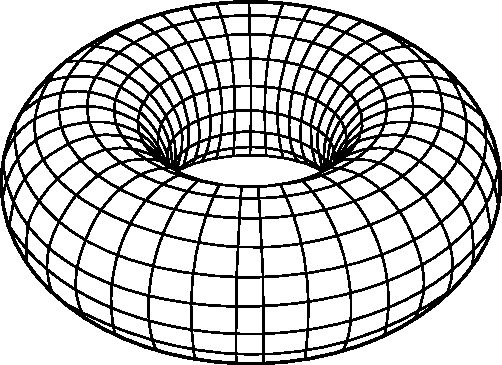
\includegraphics[width=0.8\textwidth]{torus2.pdf}
	\end{center}
\end{titlepage}
%\maketitle
\setcounter{tocdepth}{1}
\tableofcontents

\section*{Vorwort}
Dies ist ein Mitschrieb der Übung “Einführung in die Geometrie und Topologie” vom Wintersemester 2011/2012 am Karlsruher Institut für Technologie, die von Frau Dipl.-Math. Sandra Lenz gehalten wird.

\chapter{24.10.2011}

\begin{section}{Induzierte Topologie}
	\begin{definition}[Induzierte Topologie]
		Sei $X$ eine Menge. Sei $d \colon X \times X \rightarrow \R$ eine Metrik. Diese Metrik $d$ definiert durch folgende Bedingung eine Topologie $\OO$ auf $X$:
		\newline
		$O \subseteq X$ ist genau dann offen (d.h. $O \in \OO_d$), wenn für alle $x \in O$ ein $\epsilon > 0$ existiert mit
		$$
			B_\epsilon (x) := \{y \in X \mid d(x,y) < \epsilon\} \subseteq O.
		$$
		($B_\epsilon$ nennt man offenen $\epsilon$-Ball.)
	\end{definition}
\end{section}

\begin{section}{Offen und abgeschlossen}
	Sei $X$ eine Menge.
	\begin{itemize}
		\item Mengen können sowohl offen als auch abgeschlossen (zugleich) sein.
			\begin{example}
				Betrachte $\emptyset$ und $X$ in der trivialen Topologie $\OO = \{X, \emptyset\}$.
					\newline
					Es gilt: $X \in \OO, \emptyset \in \OO$ nach Definition, d.h. $X$ und $\emptyset$ sind offen.
					\newline
					Außerdem gilt: $X^c = \emptyset \in \OO$, ebenso: $\emptyset^c = X \in \OO$, d.h. die Komplemente von $X$ und $\emptyset$ sind offen und somit $X$ und $\emptyset$ abgeschlossen.
			\end{example}
			
		\item Mengen können weder offen noch abgeschlossen sein.
			\begin{example}
				Betrachte $\R$ mit der von der Standardmetrik induzierten Topologie. Es ist $[0,1[$ nicht offen in dieser Topologie, denn für den Punkt $0$ finden wir kein $\epsilon > 0$, so dass $B_\epsilon(0)$ in $[0,1[$ liegt.
				Die Menge $[0,1[$ ist aber auch nicht abgeschlossen, da ihr Komplement $\R \backslash [0,1[ = ]-\infty,0[ \cup [\underline{1},\infty[$ nicht offen ist.
			\end{example}
		\item Bilder offener Mengen unter stetigen Abbildungen müssen nicht notwendigerweise offen sein.
			\begin{example}
				Betrachte $\R$ mit der von der Standardmetrik induzierten Topologie.
				\newline
				Definiere $f \colon \R \rightarrow \R, x \mapsto x^2$.
				\newline
				Es gilt für die in $\R$ offene Menge $]-1,1[$:
				\newline
				$f(]-1,1[)=[0,1[$ und $[0,1[$ ist nicht offen in $\R$.
			\end{example}
	\end{itemize}
\end{section}

\begin{section}{Basis der von der Standardmetrik auf dem $\R^n$ definierten Topologie}
	$$\mathcal{B} = \{B_{\frac{1}{m}}(x) \mid x \in \Q^n, m \in \N\}$$
	Diese Basis ist abzählbar.
\end{section}

\begin{section}{Teilraumtopologie}
	Es sei $(X, \OO)$ ein topologischer Raum, $A \subseteq X$.
	\newline
	Die Teilraumtopologie (oder Spurtopologie) ist definiert durch
	$$\OO \big |_{A} := \{U \cap A \mid U \in \OO\} $$
	
	\begin{theorem}
		In der Tat definiert $\OO \big |_{A}$ eine Topologie auf $A$.
	\end{theorem}
	
	\begin{proof}
			$\bullet$\underline{z.z.}: Für jede Indexmenge $I$ gilt:
				$\forall i \in I \colon O_i \in \OO \big |_{A} \Rightarrow \bigcup\limits_{i \in I}{O_i} \in \OO \big |_{A}.$
			\newline
			Sei $I$ beliebige Indexmenge. Für alle $i \in I$ mit $O_i \in \OO \big |_{A}$ gilt:
			Es existieren $\mathcal{U}_i \in \OO$ mit $O_i= \mathcal{U}_i \cap A$.
			Es gilt:
			$$\bigcup\limits_{i \in I}{O_i} = \bigcup\limits_{i \in I}{(\mathcal{U}_i \cap A) } = (\bigcup\limits_{i \in I}{\mathcal{U}_i})\cap A \in \OO \big |_{A}$$ (da $\bigcup\limits_{i \in I}{\mathcal{U}_i} \in \OO$).
			\newline
			$\bullet$ \underline{z.z.}: $\forall O_1, O_2 \in \OO \big |_{A} \colon O_1 \cap O_2 \in \OO \big |_{A}.$
			\newline
			Seien $O_1, O_2 \in \OO \big |_{A}$. Dann ex. $\mathcal{U}_1, \mathcal{U}_2 \in \OO$ mit $O_i = \mathcal{U}_i \cap A, i \in \{1,2\}.$ Es gilt:
			$O_1 \cap O_2 = (\mathcal{U}_1 \cap A) \cap (\mathcal{U}_2 \cap A) = (\mathcal{U}_1 \cap \mathcal{U}_2) \cap A \in \OO \big |_{A} \text{, da } \mathcal{U}_1 \cap \mathcal{U}_2 \in \OO.$
			\newline
			$\bullet$ \underline{z.z.}: $A, \emptyset \in \OO \big |_{A}.$
			\newline
			Es gilt: $A = X \cap A \in \OO \big |_{A}\text{, da } X \in \OO$ nach Definition von $\OO$. 
			\newline
			Es gilt: $\emptyset = \emptyset \cap A \in \OO \big |_{A} \text{, da } \emptyset \in \OO$ nach Definition von $\OO$.
	\end{proof}
\end{section}

\begin{section}{Homotopieäquivalenz}
	\begin{definition}
		Seien $X,Y$ topologische Räume. $X$ heißt \underline{homotopieäquivalent zu Y}, falls es stetige Abbildungen $f \colon X \rightarrow Y$ und $g \colon Y \rightarrow X$ gibt, so dass $f \circ g \simeq id_Y$ und $g \circ f \simeq id_X$.
	\end{definition}
	
	\begin{theorem}
		$\R^n \backslash \{0\}$ ist homotopieäquivalent zur Sphäre $S^{n-1}$.
	\end{theorem}
	
	\begin{proof}
		Sei $f \colon S^{n-1} \hookrightarrow \R^n \backslash \{0\}, x \mapsto x$ (Inklusionsabbildung). Dann ist $f$ stetig.
		\newline
		Sei weiter $g \colon \R^n \backslash \{0\} \rightarrow S^{n-1}, x \mapsto \frac{x}{||x||}$. Dann ist auch $g$ stetig und es gilt:
		$g \circ f = id_{S^{n-1}}$, also insbesondere $g \circ f \simeq id_{S^{n-1}}$.
		\newline
		Für $f \circ g$ betrachte folgende Abbildung:
		$$H \colon \R^n \backslash \{0\} \times [0,1] \rightarrow \R^n \backslash \{0\}, (x,t) \mapsto (1-t) \frac{x}{||x||} + t \cdot x$$
		Dann ist $H$ stetig und es gilt für alle $x \in \R \backslash \{0\}$:
		\newline
		$H(x,1) = x = id_{\R^n \backslash \{0\}}(x)$
		\newline
		$H(x,0) = \frac{x}{||x||} = (f \circ g)(x)$
		\newline
		Dann ist $H$ Homotopie von $f \circ g$ nach $id_{\R^n \backslash \{0\}}$ (in Zeichen: $f \circ g \simeq id_{\R^n \backslash \{0\}}$).
	\end{proof}
\end{section}

\chapter{31.10.2011}
\section{Universelle Eigenschaft der Teilraumtopologie}
Es sei $(X, \OO_X)$ ein topologischer Raum und $A \subseteq X$ versehen mit der Teilraumtopologie $\OO_A = \{ O \cap A \mid O \in \OO_X \}$. 
Weiter sei $\iota \colon A \hookrightarrow X$ die Inklusionsabbildung und $(Y, \OO_Y)$ ein weiterer topologischer Raum.

\begin{theorem}{Behauptung}
Eine Abbildung $\phi \colon Y \rightarrow A$ ist genau dann stetig, wenn die Komposition $\iota \circ \phi \colon Y \rightarrow X$ stetig ist.
\end{theorem}

\begin{proof}
`$\Rightarrow$': Es sei $\phi \colon Y \rightarrow A$ stetig. [\underline{z.z.}: $\iota \circ \phi$ ist stetig, d.h. $\forall O \in \OO_X \colon (\iota \circ \phi)^{-1}(O) \in \OO_Y$]
\newline
Sei $O \in \OO_X$. Dann gilt $(\iota \circ \phi)^{-1}(O) = \phi^{-1}\left(\iota^{-1}(O)\right)$ und es ist $\iota^{-1}(O) \in \OO_A$, da $\iota$ stetig ist.
\newline
Es gilt somit $\phi^{-1}\left(\iota^{-1}(O)\right) \in \OO_Y$, da $\phi$ stetig ist (nach Voraussetzung).
\newline
`$\Leftarrow$': Es sei $\phi \colon Y \rightarrow A$ eine Abbildung, so dass $\iota \circ \phi \colon Y \rightarrow X$ stetig ist. [\underline{z.z.}: $\phi$ ist stetig, d.h. $\forall O \in \OO_A \colon \phi^{-1}(O) \in \OO_Y$.]
\newline
Sei also $O \in \OO_A$. Dann existiert $O^\prime \in \OO_X$, so dass $O = O^\prime \cap A$.
Es gilt: $\iota^{-1}(O^\prime) = O^\prime \cap A = O$.
\newline
$\phi^{-1}(O) = \phi^{-1}(O^\prime \cap A) = \phi^{-1}\left(\iota^{-1}(O^\prime)\right) = (\iota \circ \phi)^{-1}(O^\prime) \in \OO_Y$, da $\iota \circ \phi$ stetig (nach Voraussetzung).
\end{proof}

\begin{remark}{(Bemerkung in der Vorlesung)}

Die Teilraumtopologie ist die gröbste Topologie, bezüglich der die Inklusionsabbildung $\iota \colon A \hookrightarrow X$ stetig ist.
\end{remark}

\begin{proof}
\underline{Stetigkeit der Inklusionsabbildung}: [\underline{z.z.}: $\forall O \in \OO_X \colon \iota^{-1}(O) \in \OO_A$]
\newline
Sei $O \in \OO_X$. Dann gilt $\iota^{-1}(O)=O \cap A \in \OO_A$.
\end{proof}


\begin{proof}
\underline{Nichtstetigkeit in gröberen Topologien}: [\underline{z.z.}: $\OO_A \not\subseteq \tilde \OO \Rightarrow \exists O^\prime \in \OO_X \colon \iota^{-1}(O^\prime) \notin \tilde \OO$]
\newline
Sei $\OO_A \not\subseteq \tilde \OO \Rightarrow \exists O \in \OO_A\colon O \notin \tilde\OO$. Dann  $\exists O^\prime \in \OO_X \colon O = O^\prime \cap A$. Damit ist aber $\iota^{-1}(O^\prime)=O^\prime \cap A = O \notin \tilde\OO \Rightarrow \iota\colon (A,\tilde\OO) \rightarrow (X,\OO_X)$ ist nicht stetig.
\end{proof}

\section{Homöomorphismen}
Zeigen Sie, dass für $a,b \in \R$ mit $a < b$ das Intervall $(a,b)$ homöomorph zum Intervall $(0,1)$ ist, sowie dass $(0,1)$ homöomorph ist zu $\R$.
\newline
Definiere $f \colon (a,b) \rightarrow (0,1), x \mapsto \frac{a-x}{a-b}$, und $g \colon (0,1) \rightarrow (a,b), x \mapsto (1-x) \cdot a + x \cdot b$.
\newline
Es gilt für alle $x \in (a,b)$:
\newline
$(g \circ f)(x) = g \left(\frac{a-x}{a-b}\right) = \left(1- \frac{a-x}{a-b}\right)a + \frac{a-x}{a-b}b = \left(\frac{a-b-a+x}{a-b}\right)a+ \frac{a-x}{a-b}b = \frac{x-b}{a-b}a + \frac{a-x}{a-b}b = \frac{ax-ab+ab-bx}{a-b} = x$.
\newline
Es gilt für alle $x \in (0,1)$:
\newline
$(f \circ g)(x)=f\left((1-x) \cdot a + x \cdot b\right)=\frac{a-((1-x)a+bx)}{a-b}=\frac{a-a+ax-bx}{a-b}=x$. Somit ist $f$ bijektiv. 
Da $f$ und $g = f^{-1}$ stetig sind, gilt damit: $f$ ist ein Homöomorphismus, d.h. $(a,b) \equiv (0,1)$.
\newline
Definiere $h \colon (0,1) \rightarrow \R, x \mapsto \tan{\left((x-\frac{1}{2})\pi \right)}$.
\newline
\newline
$f \colon [0,1) \rightarrow S^1, t \mapsto e^{2\pi i t} \left(=(\cos{2 \pi t}, \sin{2 \pi t})\right)$ ist kein Homöomorphismus (da die Umkehrabbildung nicht stetig ist).

\begin{figure}[h]
\centering
\subfloat[$f$ ist stetig $\dots$]{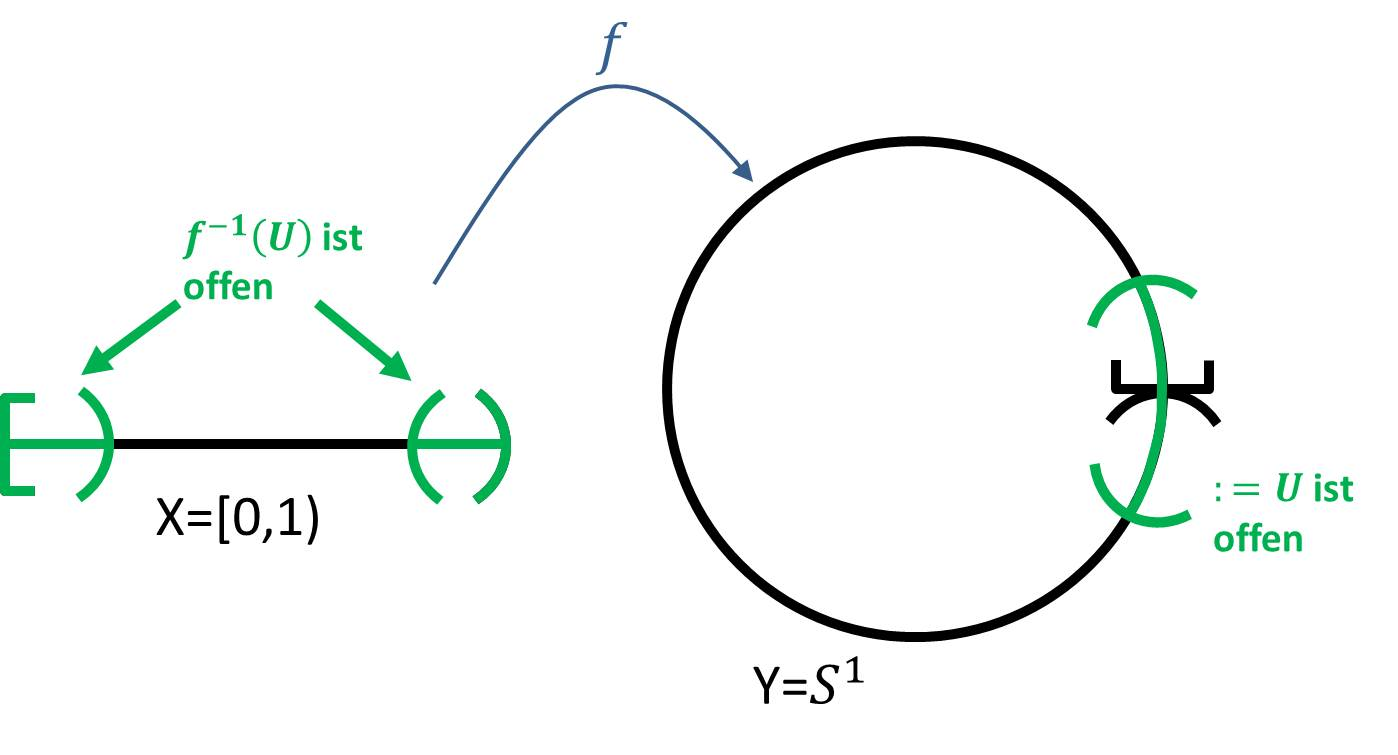
\includegraphics[width=0.75\textwidth]{images/0_1_nach_S1_f_stetig.jpg}}
\subfloat[$\dots f^{-1}$ aber nicht.]{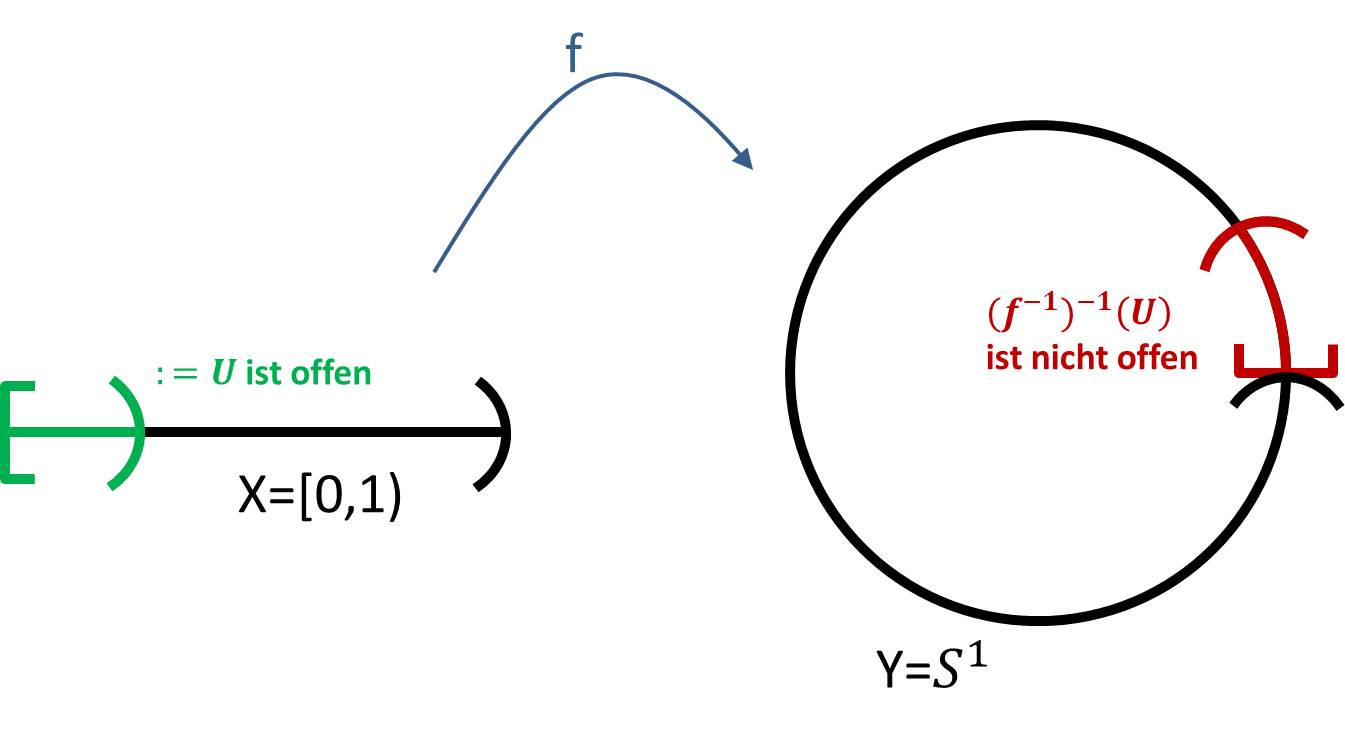
\includegraphics[width=0.75\textwidth]{images/0_1_nach_S1_f-1_nicht_stetig.jpg}}
\end{figure}

\section{Die Peano-Kurve}
(Guiseppe Peano, $\sim 1890$)
\begin{theorem}
	Es gibt eine surjektive, stetige Abbildung $I = [0,1] \rightarrow I \times I$.
\end{theorem}

\begin{figure}[h]
\centering
\subfloat[Iteration 1]{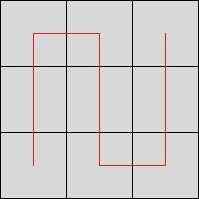
\includegraphics[width=0.4\textwidth]{images/PeanoKurve1.jpg}}\qquad
\subfloat[Iteration 2]{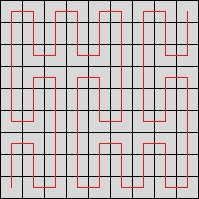
\includegraphics[width=0.4\textwidth]{images/PeanoKurve2.jpg}}
\caption{Prinzip der Peano-Kurve}
\end{figure}

\paragraph{Verallgemeinerung}
\begin{itemize}
\item Es gibt eine surjektive, stetige Abbildung $I \rightarrow I^n = I \times I \times \ldots \times I (n \in \N)$.
\item Es gibt eine surjektive, stetige Abbildung $\R \rightarrow \R^n$.
\end{itemize}

\subsection{Zugang mit Hilfe der Cantor-Menge $\mathcal{C}$}
Definiere $f \colon \mathcal{C} \rightarrow I, f \left(\sum\limits_{i=1}^{\infty}{\frac{a_i}{3}} \right) = \sum\limits_{i=1}^{\infty}{\frac{\frac{a_i}{2}}{2^i}}$ für $a_i \in \{0,2\}$.
\newline
Dann ist $f$ surjektiv und stetig.
\newline
Definiere $g \colon \mathcal{C} \rightarrow \mathcal{C} \times \mathcal{C}, g \left(\sum\limits_{i=1}^{\infty}{\frac{a_i}{3}} \right) = \left(\sum\limits_{i=1}^{\infty}{\frac{a_{2i}}{3^i}}, \frac{a_{2i+1}}{3^i} \right)=:(g_1,g_2)$ für $a_i \in \{0,2\}$.
\newline
Dann ist $g$ surjektiv und stetig.
\newline
Es ist auch $h \colon \mathcal{C} \rightarrow I \times I, x \mapsto \left(f(g_1(x)), f(g_2(x))\right)$ surjektiv und stetig.
\newline
Setze die Abbildung $h$ durch lineare Fortsetzungen stetig auf $I$ fort.

\chapter{07.11.2011}
\section{Nachträge und Wiederholungen zur Vorlesung}
\subsection{Überdeckung, Teilüberdeckung und Kompaktheit}
Sei $X$ ein topologischer Raum.
\begin{definition}
	\begin{itemize}
		\item Eine Familie $\{\mathcal{U}_\alpha \mid \alpha \in A \}$ von Teilmengen von $X$ heißt \underline{Überdeckung} von $X$, falls gilt: $X = \bigcup\limits_{\alpha \in A}{\mathcal{U}_\alpha}$.
		\item Eine Überdeckung heißt \underline{offen} (bzw. \underline{abgeschlossen}), falls alle $\mathcal{U}_\alpha (\alpha \in A)$ offen (bzw. abgeschlossen) sind.
		\item Es heißt $X$ \underline{kompakt}, falls jede offene Überdeckung $\mathcal{U}=\{U_\alpha, \alpha \in A\}$ eine endliche Teilüberdeckung $\mathcal{U}^\prime$ besitzt, d.h. es existiert $A^\prime \subset A$ endlich, so dass $\mathcal{U}^\prime = \{\mathcal{U}_\alpha \mid \alpha \in A^\prime \}$ eine offene Überdeckung von $X$ ist.
	\end{itemize}
\end{definition}

\begin{example}
	\begin{itemize}
		\item Endliche Räume und mit der trivialen Topologie versehene Räume sind kompakt.
		\item Diskrete Räume sind genau dann kompakt, wenn sie aus endlich vielen Elementen bestehen.
		\item $\R$ (versehen mit der Standardtopologie) ist \underline{nicht} kompakt, $\R_{\mathcal{T}_1}$ schon. ($\mathcal{T}_1 = \{ \R \backslash E \mid E \text{ endliche Teilmenge von } \R \} \cup \{\emptyset\}$)
	\end{itemize}
\end{example}

\begin{definition}	Eine \underline{kompakte Menge} ist eine Teilmenge eines vom Kontext her klaren topologischen Raumes, die bezüglich der Teilraumtopologie kompakt ist.
\end{definition}

\begin{example}
	$[0,1) (\subseteq \R)$ ist nicht kompakt, \underline{denn:} Die Überdeckung $\{(-1,1-\frac{1}{n}) \mid n \in \N \}$ von $[0,1)$ enthält keine endliche Teilüberdeckung.
\end{example}

\begin{remark}
	\begin{itemize}
		\item \underline{Satz von Heine-Borel:} Teilmengen euklidischer, endlich dimensionaler Räume sind genau dann kompakt, wenn sie abgeschlossen und beschränkt sind.
		\item Abgeschlossene Teilmengen kompakter Räume sind kompakt.
		\item Stetige Bilder kompakter Mengen sind kompakt, d.h. ist $X$ eine kompakte Menge, $Y$ topologischer Raum, $f \colon X \rightarrow Y$ stetig, dann ist $f(X)$ kompakt.
		\item Ist $X$ kompakt, $f \colon X \rightarrow \R$ stetig, so ist $f(X)$ kompakt und $f$ nimmt auf $X$ Maximum und Minimum an.
		\item \underline{Lebesque-Lemma:} Ist $f \colon X \rightarrow Y$ stetige Abbildung topologischer Räume und $X$ metrisch und kompakt, so gilt:
		\newline
			Ist $\mathcal{U}$ eine offene Überdeckung von $Y$, so existiert $\delta \in \R_{>0}$, sodass für alle $A \subseteq X$ mit diam $A < \delta$ ein $U^\prime \in \mathcal{U}$ mit $f(A) \subseteq U^\prime$ existiert.
	\end{itemize}
\end{remark}

\subsection{Wegzusammenhang}
\begin{definition}
	\begin{itemize}
		\item Ein \underline{Weg} in $X$ ist eine stetige Abbildung $\gamma \colon I(=[0,1]) \rightarrow X$ mit Anfangspunkt $\gamma(0)$ und Endpunkt $\gamma(1)$.	
		\item Man nennt $X$ \underline{wegzusammenhängend}, falls für alle $x,y \in X$ ein Weg $\gamma \colon [0,1] \rightarrow X$ in $X$ existiert mit $\gamma(0)=x, \gamma(1)=y$.
		\item Eine \underline{Wegzusammenhangskomponente} von $X$ ist eine wegzusammenhängende Teilmenge von $X$, die in keiner echt größeren solchen Teilmenge enthalten ist.
	\end{itemize}
\end{definition}

\begin{remark}
	\begin{itemize}
		\item Jeder Punkt von $X$ liegt in genau einer Wegzusammenhangskomponente von $X$, und zwei solche Komponenten sind entweder gleich oder disjunkt.
		\item Stetige Bilder wegzusammenhängender Mengen sind wegzusammenhängend.
	\end{itemize}
\end{remark}

\begin{corollary}
	Wegzusammenhang bleibt unter Homöomorphismen erhalten, ebenso die Anzahl der Wegzusammenhangskomponenten.
\end{corollary}

Wegzusammende topologische Räume sind zusammenhängend (Übungsaufgabe), die Umkehrung gilt im Allgemeinen nicht.

\paragraph{Beispiel eines Raumes, der zusammenhängend, aber nicht wegzusammenhängend ist}
(TODO: Bild)
\newline
Definiere $A = \{(x,y) \in \R^2 \mid x > 0, y = \sin{\left(\frac{1}{x}\right)}\}, X := A \cup \{(0,0)\}$.
\newline
Es gilt:
\begin{itemize}
	\item Es ist $A$ wegzusammenhängend, denn:
	 \newline	
	 $A \cong (0, +\infty) \cong \R$, und $\R$ ist wegzusammenhängend.
	\item Es ist $X$ zusammenhängend, denn:
		\newline
		Es gilt: $\bar{A} = A \cup \{(0,y) \mid y \in [-1,1]\}$ ist als Abschluss einer zusammenhängenden Menge wieder zusammenhängend (siehe Bemerkung in der Vorlesung).
		\newline
		Außerdem gilt: $A \subseteq X \subseteq \bar{A}$, und $X$ ist als Teilmenge des Abschlusses eines zusammenhängenden Raumes wieder zusammenhängend. (\underline{Allgemein:} Es sei $A$ zusammenhängend, $A \subseteq B \subseteq \bar{A}$. Dann ist auch $B$ zusammenhängend.)
	\item Es ist $X$ \underline{nicht wegzusammenhängend}, denn:
		\newline
		Es lässt sich $(0,0)$ nicht über einen Weg in $X$ mit einem beliebigen anderen Punkt aus $X$ verbinden\footnote{Formale Begründung: Jeder in $(0,0)$ startende Weg ist konstant.}.
\end{itemize}

\begin{remark}
	Der Abschluss wegzusammenhängender Räume ist im Allgemeinen nicht wegzusammenhängend!
\end{remark}

\begin{example}[Beispiel von oben]
	Der Abschluss von $A$ \underline{in $X$} - nicht in $\R^2$ - ist $X$, und $X$ ist (s.o.) nicht wegzusammenhängend.
\end{example}

\begin{remark}
	Besitzt jeder Punkt eines topologischen Raumes $X$ eine wegzusammenhängende Umgebung, so sind alle Wegzusammenhangskomponenten offen in $X$, und $X$ ist genau dann wegzusammenhängend, wenn $X$ zusammenhängend ist.
\end{remark}

\begin{example}
	Offene Teilmengen von $\R^n$ sind genau dann wegzusammenhängend, wenn sie zusammenhängend sind, \underline{denn:}
	\newline
	Jeder Punkt $x \in \R^n$ besitzt dann als offene Umgebung einen offenen Ball, und offene Bälle sind wegzusammenhängend.
\end{example}

\chapter{14.11.2011}
\section{Beispiele für Beweise im Kontext von Hausdorffräumen}
\begin{theorem}{Behauptung:}
Ist $X$ ein Hausdorffraum, so besitzt jede Folge $(x_n)_{n \in \N} \in X^\N$ höchstens einen Grenzwert.
\end{theorem}
\begin{proof}
	Sei $X$ ein Hausdorffraum.
	\newline
	\underline{Annahme:} Es existiert eine Folge $(x_n)_{n \in \N} \in X^\N$ mit $x = \lim\limits_{n \rightarrow \infty}(x_n) = x^\prime$ und $x \neq x^\prime$.
	\newline
	Da $X$ Hausdorffsch ist, existieren offene Teilmengen $U,V \subseteq X$, mit $U \cap V = \emptyset$ und $x \in U, x^\prime \in V$. Dann existieren $n_0, n_0^\prime \in \N$ mit $x_n \in U, x_m \in V \text{ für alle } n \in \N_{\geq n_0}, m \in \N_{\geq n_0^\prime}$. Dann gilt also für alle $k \geq \max\{n_0,n_0^\prime\} \colon x_k \in U \cap V=\emptyset$. $\lightning$
\end{proof}

\begin{theorem}
Jeder metrische Raum ist Hausdorffsch.
\end{theorem}

\begin{proof}
[\underline{z.z.:} $\forall x\neq y \in X \exists U_x, U_y \subseteq X \colon U_x \cap U_y = \emptyset$.]
Seien $x\neq y \in X$. Wähle $U_x := B_\frac{d(x,y)}{3}(x), U_y := B_\frac{d(x,y)}{3}(y)$.
\newline
Dann gilt: $U_x \cap U_y = \emptyset$.
\end{proof}

\section{Beispiele für Mannigfaltigkeiten}
\begin{enumerate}
	\item Was sind 0-dimensionale Mannigfaltigkeiten?
		\begin{itemize}
			\item Abzählbare diskrete Mengen.
		\end{itemize}
		
	\item \underline{1-dimensionale glatte Mannigfaltigkeiten} (TODO: Bild 1)
		\begin{itemize}
			\item Offene Intervalle in $\R$ sind 1-dimensionale glatte Mannigfaltigkeiten, \underline{denn:} Seien $a,b \in \R$ mit $a < b$.
			\begin{itemize}
				\item $(a,b)$ ist als metrischer Raum Hausdorffsch.
				\item Es ist $\mathcal{B} = \{B_{\frac{1}{n}}(x) \mid x \in \Q, n \in \N\}$ eine abzählbare Basis der Topologie.
				\item $(a,b)$ ist lokal homöomorph zu $\R$, \underline{denn:} Es gilt: $id \colon (a,b) \mapsto (a,b) \subseteq \R$ ist ein Homöomorphismus einer offenen Menge in eine offene Teilmenge von $\R$. Somit ist $\left((a,b),id_{(a,b)}\right)$ eine (\underline{globale})\footnote{Global, da für die ganze Mannigfaltigkeit gleich.} Karte.
				\item Für den Kartenwechsel gilt: $id_{(a,b)} \circ id_{(a,b)}^{-1} \colon (a,b) \rightarrow (a,b), x \mapsto x$, ist eine glatte Abbildung.
			\end{itemize}
		
		\item $S^1 = \{ x \in \R^2 \mid ||x|| = 1\}$ ist eine 1-dimensionale glatte Mannigfaltigkeit (TODO Bild 2), \underline{denn:}
			\begin{itemize}
				\item Es ist $S^1$ als Teilmenge des metrischen Raumes $\R^2$ Hausdorffsch.
					\newline
					Ebenso besitzt $S^1$ eine abzählbare Basis der Topologie.
				\item Definiere $$U_1 := \{(x,y) \in S^1 \mid y \neq 1\} = S^1 \backslash \{N\} \quad \left(N := (0,1)\right)$$ und $$U_2 := \{(x,y) \in S^1 \mid y \neq -1\} = S^1 \backslash \{S\} \quad \left(S := (0,-1)\right).$$
				Dann gilt:
				\item $U_1 \cup U_2 = S^1$,
				\item Es sind $U_1$ und $U_2$ offene Teilmengen von $S^1$, denn sie sind jeweils Komplement einer einpunktigen und damit abgeschlossenen Menge.
				\item Definiere $$\varphi_1 \colon U_1 \rightarrow \R, (x,y) \mapsto \frac{x}{1-y},$$
				$$\varphi_2 \colon U_2 \rightarrow \R, (x,y) \mapsto \frac{x}{1+y}.$$
				Im Folgenden zeigen wir, dass $(U_1, \varphi_1)$ eine Karte ist. Analoges gilt auch für $(U_2, \varphi_2)$ mit analoger Rechnung.
				\item Definiere $$\psi \colon \R \rightarrow S^1, u \mapsto (\frac{2u}{u^2+1}, \frac{u^2-1}{u^2+1}).$$
				Dann gilt:
				$$\varphi_1 \circ \psi = id_\R,$$
				$$\psi \circ \varphi_1 = id_{U_1}.$$
				Damit ist $\varphi_1$ bijektiv.
				\newline
				Da $\varphi_1$ und $\psi$ stetig sind, ist $\varphi_1$ damit ein Homöomorphismus.
				\item Die Kartenwechsel sind glatt, denn es gilt:
				$$\varphi_1(U_1 \cap U_2) = \R \backslash \{0\} = \varphi_2(U_1 \cap U_2).$$
				Für alle $u \in \R \backslash \{0\}$ gilt:
				$$(\varphi_2 \circ \varphi_1^{-1})(u) = (\varphi_2 \circ \psi)(u) = \frac{1}{u},$$
				und dies ist tatsächlich ein $C^\infty-$Diffeomorphismus\footnote{d.h. bijektiv und unendlich oft differenzierbar und mit unendlich oft differenzierbarer Umkehrabbildung} $\R \backslash \{0\} \rightarrow \R \backslash \{0\}$.
			\end{itemize}
	\end{itemize}			
	
	\item Es ist $\R^n$ eine $n$-dimensionale glatte Mannigfaltigkeit, \underline{denn:}
		\begin{itemize}
			\item $\R^n$ ist Hausdorffsch und besitzt eine abzählbare Basis der Topologie.
			\item $(\R^n, id_{\R^n})$ ist eine globale Karte.
		\end{itemize}
\end{enumerate}

\begin{remark}
	Jeder Atlas, der aus nur einer Karte besteht, ist glatt.
\end{remark}

\begin{proof}
	Es sei $\mathcal{A} = \{(\varphi,U)\}$ dieser Atlas. Dann gilt:
	\newline
	Es gibt nur genau einen Kartenwechsel: 
	$$\varphi \circ \varphi^{-1} = id_{\varphi(U)} \colon \varphi(U) \rightarrow \varphi(U)$$ und dieser ist natürlich glatt.
\end{proof}

\begin{theorem}
	Offene Teilmengen von $C^k$-Mannigfaltigkeiten sind wieder $C^k$-Mannigfaltigkeiten.
\end{theorem}

\begin{proof}
	Es sei $M$ eine $C^k$-Mannigfaltigkeit der Dimension $n$, $N \subseteq_{offen} M$.
	\begin{itemize}
		\item Als Teilmenge von $M$ ist $N$ Hausdorffsch und auch die abzählbare Basis der Topologie überträgt sich.
		\item Es sei $\mathcal{A} = \{(\varphi_\alpha, U_\alpha) \mid \alpha \in \Lambda \}$ ($\Lambda$ Indexmenge) ein $C^k$-Atlas von $M$.
		\newline
		Für alle $\alpha \in \Lambda$ ist $U_k \cap N$ offen in $N$ und es gilt:
		$$\varphi_\alpha \big |_{U_\alpha \cap N} \colon U_\alpha \cap N \rightarrow \varphi_\alpha(U_\alpha \cap N) \subseteq \R^n$$
		und $\varphi_\alpha(U_\alpha \cap N)$ ist als stetiges Bild der offenen Menge $U_\alpha \cap N$ wieder offen.
		\newline
		Somit ist $\{(\varphi_\alpha \big |_{U_\alpha \cap N}, U_\alpha \cap N) \mid \alpha \in \Lambda\}$ ein Atlas für $N$.
		\newline
		Da die Kartenwechsel weiterhin $C^k$-Abbildungen sind, ist dieser Atlas ein $C^k$-Atlas für $N$.
	\end{itemize}
\end{proof}

\begin{example}
	Es gilt: $GL(n,\R) = \det^{-1}(\R \backslash \{0\}) \subseteq_{offen} \R^{n^2}$
\end{example}

\chapter{21.11.11}

\section{Untermannigfaltigkeiten}
\begin{theorem}{$C^\infty$-Untermannigfaltigkeiten von $\R^{n+l}$ sind $C^\infty$-Mannigfaltigkeiten}
	Es sei $M \subseteq \R^{n+l}$ eine $n$-dimensionale $C^\infty$-Untermannigfaltigkeit von $\R^{n+l}$, versehen mit der Teilraumtopologie, und $\{\psi_\alpha \colon W_\alpha \rightarrow U_\alpha \cap M\ \mid \alpha \in \Lambda\}$ eine Menge lokaler Parametrisierungen (siehe Untermannigfaltigkeitskriterium, (c)) mit $M \subseteq \bigcup\limits_{\alpha \in \Lambda}{U_\alpha}$.
	\newline
	Dann ist $\mathcal{A}=\{(\psi_\alpha^{-1}, U_\alpha \cap M) \mid \alpha \in \Lambda\}$ ein $C^\infty$-Atlas für $M$ und somit eine $C^\infty$-Mannigfaltigkeit.
\end{theorem}

\begin{proof}
	\begin{itemize}
		\item Es gilt: $M$ ist Hausdorffsch und besitzt eine abzählbare Basis der Topologie als Teilmenge von $\R^{n+l}$.
		\item Es ist $\mathcal{A}$ ein Atlas (nach Definition der lokalen Parametrisierungen).
		\item $[$\underline{z.z.:} Die Kartenwechsel sind glatt, d.h.: 
			$$\forall \alpha, \beta \in \Lambda \colon (U_\alpha \cap M) \cap (U_\beta \cap M) \neq \emptyset$$
			$$\Rightarrow \psi_\beta^{-1} \circ \psi_\alpha \colon \psi_\alpha^{-1}(U_\alpha \cap U_\beta \cap M) \rightarrow \psi_\beta(U_\alpha \cap U_\beta \cap M)$$
			 ist glatt.$]$
			Seien $\alpha, \beta \in \Lambda$ mit $(U_\alpha \cap M) \cap (U_\beta \cap M) \neq \emptyset$.
			\newline
			(\underline{Vorsicht:} Es ist $\psi_\beta^{-1}$ nicht auf einer offenen Teilmenge von $\R^{n+l}$ definiert, daher ist die Kettenregel nicht direkt anwendbar!)
			\newline
			\underline{Zeige:} Es ist $\psi_\beta^{-1}$ auf einer (offenen) Umgebung eines jeden Punktes $y \in U_\alpha \cap U_\beta \cap M$ eine glatte Abbildung.
			\newline
			Sei $x \in \psi_\alpha^{-1}(U_\alpha \cap U_\beta \cap M)$. Nach dem Untermannigfaltigkeits-Kriterium (b) existiert eine Umgebung $U \subseteq U_\alpha \cap U_\beta$ von $\psi_\alpha(x) \in M$ in $\R^{n+l}$ und ein $C^\infty$-Diffeomorphismus $\varphi \colon U \rightarrow \varphi(U) \subseteq \R^{n+l}$ mit $\varphi(U \cap M) = \varphi(U) \cap (\R^{n} \times \{0\})$
			\newline
			Definiere $\pi \colon \R^{n+l} \cong \R^n \times \R^l \rightarrow \R^n$, die Projektion auf die ersten $n$ Komponenten und $\iota \colon \R^n \rightarrow \R^{n+l}, x \mapsto (x,0)$, die Inklusion. Dann gilt auf $\varphi(U \cap M) \subseteq \R^{n} \times \{0\}$: $\iota \circ \pi = id$. Daher gilt auf $\psi_\alpha^{-1}(U \cap M)$: 
			$$\psi_\beta^{-1} \circ \psi_\alpha = \psi_\beta^{-1} \circ \varphi^{-1} \circ \varphi \circ \psi_\alpha = (\psi_\beta^{-1} \circ \varphi^{-1} \circ \iota)\circ(\pi \circ \varphi \circ \psi_\alpha).$$
			Es sind $(\psi_\beta^{-1} \circ \varphi^{-1} \circ \iota) = (\pi \circ \varphi \circ \psi_\beta)^{-1}$ und $\pi \circ \varphi \circ \psi_\alpha$ glatte Abbildungen zwischen offenen Teilmengen des $\R^n$ und somit auch die Komposition $\psi_\beta^{-1} \circ \psi_\alpha$.
	\end{itemize}
\end{proof}

\section{Wichtige Spezialfälle (und Beispiele) von Untermannigfaltigkeiten}
\paragraph{(a) Niveaumengen}
Es seien $V \subseteq \R^{n+l}$ offen, $f \in C^\infty(V,\R^l), c \in \R^l$. Gilt Rang $Df(x)=l$ in jedem Punkt $x$ der Niveaumenge
$$f^{-1}(c) = \{x \in V \mid f(x) = c\},$$
so ist $f^{-1}(c)$ eine $n$-dimensionale glatte Untermannigfaltigkeit von $\R^{n+l}$.

\begin{proof}
	Wende Untermannigfaltigkeits-Kriterium (a) auf die Abbildung $$g = f - c \colon x \mapsto f(x)-c$$ an.
	\newline
	$[$\underline{z.z.:} Rang $Df(x)=l$ auf einer Umgebung $U$ von $f^{-1}(c)$, nicht nur auf der Niveaumenge selbst!$]$
	\newline
	Sei $x_0 \in f^{-1}(c)$. Da Rang $Df(x_0) = l$, existiert eine $(l \times l)$-Unterdeterminante $A(x)$ von $\det{Df(x)}$, so dass $A(x_0)\neq \emptyset$. Da $f$ stetig ist, ist die Abbildung $x \mapsto A(x)$ stetig, und somit folgt: $A(x)\neq 0$ auf einer Umgebung $U(x_0)$ von $x_0$. Dann ist Rang $Df(x)=l$ für alle $x \in U(x_0)$.
	\newline
	Setze $U:= \bigcup\limits_{x_0 \in f^{-1}(c)}{U(x_0)}$, dann folgt die Behauptung.
\end{proof}

\begin{example}
	(TODO:Bild)
	\newline
	Der \underline{Zylinder} $M=\{(x,y,z) \in \R^3 \mid x^2+y^2 = 1\}$ ist als Niveaumenge der Abbildung $f \colon \R^3 \rightarrow \R, (x,y,z) \mapsto \underbrace{x^2+y^2}-1$, eine $C^\infty$-Untermannigfaltigkeit von $\R^3$.
\end{example}

\paragraph{(b)}
\begin{example}
	Der Graph der Abbildung $\varphi \colon \R \rightarrow \R^2, t \mapsto (\cos{(t)},\sin{(t)})$, d.h. die Menge $\{(\cos{(t)},\sin{(t)},t) \mid t \in \R\}$, die \underline{Helix}
	(TODO: Bild), ist eine 1-dimensionale glatte Untermannigfaltigkeit von $\R^3$.
\end{example}

\paragraph{(c) Global parametrisierte Untermannigfaltigkeiten}
Es sei $W \subseteq \R^n$ offen und $\psi \colon W \rightarrow \R^{n+l}$ glatt mit Rang $D\psi(w)=n$ für alle $w \in W$. Es sei ferner $\psi \colon W \rightarrow \psi(W)$ Homöomorphismus.
Dann ist $\psi(W)$ eine $C^\infty$-Untermannigfaltigkeit von $\R^{n+l}$ (nach Untermannigfaltigkeits-Kriterium (c) mit $U := \R^{n+l}$).
\newline
Für $n=2$ und $l=1$ heißt $\psi(W)$ eine \underline{parametrisierte Fläche} von $\R^3$.

\begin{example}
	\begin{enumerate}
		\item Parametrisierung des Zylinders:
			\newline
			Betrachte die glatte Abbildung $\psi \colon (0, 2 \pi) \times \R \rightarrow \R^3, (t,s) \mapsto (\cos{(t)}, \sin{(t)}, s)$. Das Bild dieser Abbildung ist der Zylinder im $\R^3$ (wie oben, ohne eine Gerade).
			Es gilt:
			$$D\psi(t,s) = \begin{pmatrix} -\sin{(t)} & 0 \\ \cos{(t)} & 0 \\ 0 & 1  \end{pmatrix} $$ für alle $(t,s) \in \R^2$, und damit:
			Rang $D \psi(t,s)=2$ für alle $(t,s) \in \R$, da $\sin$ und $\cos$ keine gemeinsamen Nullstellen haben.
			\newline
			Damit ist $\psi$ eine (globale) Parametrisierung des Zylinders.
			
		\item (Rotationsflächen im $\R^3$)
			\newline
			Rotiere für Konstanten $0 < r < a$ die Kurve $\gamma \colon [0,2\pi] \rightarrow \R^3, t \mapsto (a + r \cdot \cos{(t)}, 0, r \cdot \sin{(t)})$.
			(TODO: Bild) in der $x_1 x_3$-Ebene:
			$$\begin{pmatrix}
				x \\ y \\z
			\end{pmatrix} = \begin{pmatrix}
			\cos{\Theta} & -\sin{\Theta} & 0 \\ \sin{\Theta} & \cos{\Theta} & 0 \\ 0 & 0 & 1
\end{pmatrix} \begin{pmatrix}
	a + r \cdot \cos{(t)} \\ 0 \\ r \cdot \sin{(t)}
\end{pmatrix}$$

	$$= \underbrace{\begin{pmatrix}
	(a + r \cdot \cos{(t)}  \cos{(\Theta)} \\ (a + r \cdot \cos{(t)})  \sin{(\Theta)} \\ r \cdot \sin{(t)}
	\end{pmatrix} }_{(*)}$$
	Dann definiert $\Phi_\gamma \colon (0, 2\pi) \times (0, 2 \pi) \rightarrow \R^3, (\Theta, t) \mapsto (*)$
	eine parametrisierte Fläche, den Rotationstorus.
	\newline
	$\bullet$ Der Rotationstorus $T \subseteq \R^3$ lässt sich als Niveaumnge definieren: 
	$$T = \{(x,y,z) \in \R^3 \mid z^2 + (\sqrt{x^2+y^2}-a)^2 = r^2\}.$$
	$\bullet$ Eine weitere (aus der Vorlesung bekannte) Darstellung des Torus ist
	$$S^1 \times S^1 = \{(x_1,x_2,x_3,x_4) \in \R^4 \mid (x_1)^2 + (x_2)^2 = 1 \wedge (x_3)^2 + (x_4)^2 = 1 \},$$
	und dies ist nicht die letzte Möglichkeit der Darstellung des Torus (siehe nächste Vorlesung) \ldots 
	\end{enumerate}
\end{example}

\end{document}
